\documentclass[12pt,a4paper]{article}

% Required packages for math and images
\usepackage{amsmath, amssymb, amsthm}
\usepackage{graphicx}
\usepackage{geometry}
\usepackage{float} % For better figure placement
\geometry{top=3cm, bottom=3cm, left=2.5cm, right=2.5cm}

\begin{document}

% --- Custom Title Page matching the provided layout ---
\begin{titlepage}
    \centering
    \vspace*{0.5cm}
    
    {\small In the Name of God} \\[2cm]
    
    % The logo image saved as sharif_logo.png
    
\includegraphics[width=4.5cm]{sharif_logo.png} \\[2cm]
    
    {\Large Probability and Statistics in Engineering Project} \\[1.5cm]
    
    {\Huge \textbf{Multi-Armed Bandit}} \\[3cm]
    
    {\large Instructor:} \\[0.3cm]
    {\Large Dr. Mohammad Hossein Yasaei Meybodi} \\[2cm]
    
    {\large Group Members:} \\[0.2cm]
    {\large Seyed Kiarash Eshraghi Naeini \quad Seyed Mohammad Moein Hosseini} \\[2cm]
    
    {\large Department of Electrical Engineering} \\[0.2cm]
    {\large Sharif University of Technology}
    
    \vfill
    
    %{\large 1404}
    %\vspace*{1cm}
\end{titlepage}
% --- End of Title Page ---

\newpage

\section*{Theory Question 1} %
\textbf{Example 1: Drugs and Patients}
\begin{itemize}
    \item \textbf{a) Arm:} The drug (since drugs possess a certain level of effectiveness, which is modeled as a random variable).
%
    \item \textbf{b) Reward:} The effectiveness of the drug (which can take any real value).
%
    \item \textbf{c) Round:} Each instance of administering a drug to a patient.
%
    \item \textbf{d) 1. Exploitation:} Exploitation here differs slightly from our main problem.
Generally, we want to select arms over $T$ rounds to maximize the total reward.
Here, we aim to minimize the number of rounds required to reach a specific level of effectiveness.
%
    \item \textbf{d) 2. Exploration:} This implies allocating a certain number of experimental rounds ($T'$) to test less-frequently used drugs.
If we solely explore, the total number of rounds increases significantly, which is undesirable.
Conversely, pure exploitation prevents accurate medical comparisons regarding drug efficacy.
%
\end{itemize}

\textbf{Example 2: Advertisements}
\begin{itemize}
    \item \textbf{a) Arm:} The advertisement (our goal is to maximize total clicks over $T$ ad display stages).
%
    \item \textbf{b) Reward:} A user click (a binary variable: 0 for no click, 1 for a click).
%
    \item \textbf{c) Round:} The number of times the ad is displayed to users.
%
    \item \textbf{d) 1. Exploitation:} Focusing purely on the ad that has accumulated the most clicks over $T'$ rounds.
%
    \item \textbf{d) 2. Exploration:} Displaying less-tested ads to users during $T$ rounds.
Pure exploitation might negatively impact user experience due to repetition.
Pure exploration might annoy users with irrelevant ads, ultimately decreasing the total click rate.
%
\end{itemize}

\textbf{Example 3: Movie Recommendations}
\begin{itemize}
    \item \textbf{a) Arm:} Movie categories or specific movies (aiming to maximize positive feedback over $T$ viewing rounds).
%
    \item \textbf{b) Reward:} User feedback (a function of watch time or explicit likes/dislikes).
%
    \item \textbf{c) Round:} The number of times a movie is suggested to the user.
%
    \item \textbf{d) 1. Exploitation:} Primarily suggesting highly viewed or highly rated movie categories.
%
    \item \textbf{d) 2. Exploration:} Recommending movie categories that the user has rarely seen.
Without exploration, the user might grow bored of the repetitive content.
Without exploitation, the user might be overwhelmed with irrelevant suggestions and become dissatisfied.
%
\end{itemize}

\section*{Theory Question 2} %
Based on the problem description, we model the scenario as a Multi-Armed Bandit problem: %
\begin{itemize}
    \item \textbf{a) Arm:} Movie Genre (we want to maximize the rating over $T$ movie-watching rounds/days).
%
    \item \textbf{b) Reward:} Rating (taking discrete values from 0 to 5).
%
    \item \textbf{c) Round:} The number of times the student watches a movie during the semester.
%
    \item \textbf{d) 1. Exploitation:} Choosing the genre that has received the highest average rating so far.
%
    \item \textbf{d) 2. Exploration:} Diversifying selections by choosing less-watched genres.
%
\end{itemize}

A purely exploitative strategy would be: if the Action genre receives the highest rating in the first 5 rounds, we exclusively watch Action movies thereafter.
However, the student might eventually get tired of this genre, and we might ignore other untested genres that could potentially yield even higher ratings, thus failing to maximize overall satisfaction.
%
A purely exploratory strategy involves constantly trying new or unseen genres.
Obviously, not all genres will be appealing, leading to suboptimal total ratings over the semester.
%

Intuitively, an interactive, alternating approach between exploration and exploitation is required.
For example, exploring for $T'$ rounds, then exploiting the best genre for $T''$ rounds, and subsequently returning to exploration if the ratings for the exploited genre begin to decline over time.
%

\section*{Theory Question 3} %
If we know that the $i$-th arm is chosen at round $t$, and it is the $s$-th time this arm is pulled, we have: %
\[
\mathbb{E}[r_t | A_t = i] = \mathbb{E}[X_{i,s}] = \mu_i
\]
Because if the $i$-th arm is selected, our reward is $X_{i,s}$.
%
Suppose $T_r$ is the set of indices $t$ where the indicator function is 1, meaning $A_t = i$.
Then: %
\[
N_i(T) = \sum_{t=1}^T \mathbb{I}\{A_t = i\} = \sum_{t \in T_r} 1 + \sum_{t \notin T_r} 0 = |T_r|
\] %
This definition is intuitively logical because the size of the set $T_r$ represents the total number of times the indicator $A_t$ equals 1 (i.e., arm $i$ is chosen).
%

From the previous equations, the expected cumulative reward is: %
\[
\mathbb{E}[S_T] = \mathbb{E}\left[ \sum_{t=1}^T r_t \right] = \sum_{t=1}^T \mathbb{E}[r_t]
\] %
For the expected value of $r_t$: %
\[
\mathbb{E}[r_t] = \sum_{i=1}^k \mathbb{E}[r_t | A_t = i] \times P(A_t = i)
\] %
\[
\mathbb{E}[N_i(T)] = \mathbb{E}\left[ \sum_{t=1}^T \mathbb{I}\{A_t = i\} \right] = \sum_{t=1}^T \mathbb{E}[\mathbb{I}\{A_t = i\}] = \sum_{t=1}^T P(A_t = i)
\] %
Therefore, we obtain: %
\[
\mathbb{E}[S_T] = \sum_{t=1}^T \sum_{i=1}^k \mu_i \times P(A_t = i) = \sum_{i=1}^k \mu_i \mathbb{E}[N_i(T)]
\] %

\section*{Theory Question 4} %
\[
\mathbb{E}[\hat{\mu}_{i,n}] = \mathbb{E}\left[ \frac{1}{n} \sum_{s=1}^n X_{i,s} \right] = \frac{1}{n} \sum_{s=1}^n \mathbb{E}[X_{i,s}] = \mu_i
\] %
\[
\mathrm{Var}(\hat{\mu}_{i,n}) = \mathrm{Var}\left( \frac{1}{n} \sum_{s=1}^n X_{i,s} \right) = \frac{1}{n^2} \sum_{s=1}^n \mathrm{Var}(X_{i,s}) = \frac{\mu_i(1-\mu_i)}{n}
\] %
By Chebyshev's inequality, for any $\varepsilon>0$: %
\[
P\left(|\hat{\mu}_{i,n} - \mu_i| \geq \varepsilon\right) \leq \frac{\mathrm{Var}(\hat{\mu}_{i,n})}{\varepsilon^2} = \frac{\mu_i(1-\mu_i)}{n \varepsilon^2}
\] %
This relation holds for any $\varepsilon \in \mathbb{R}^+$.
As $n$ grows arbitrarily large: %
\[
0 \leq \lim_{n \to \infty} P\left(|\hat{\mu}_{i,n} - \mu_i| \geq \varepsilon\right) \leq \lim_{n \to \infty} \frac{\mu_i(1-\mu_i)}{n \varepsilon^2} = 0
\] %
\[
\implies \lim_{n \to \infty} P\left(|\hat{\mu}_{i,n} - \mu_i| \geq \varepsilon\right) = 0
\] %
Thus, the sample mean converges in probability to the true mean (the weak law of large numbers).
%

\section*{Theory Question 5} %
\[
\mathbb{E}[S_T] = \sum_{i=1}^k \mu_i \mathbb{E}[N_i(T)]
\] %
The number of times the optimal arm is pulled in an ideal scenario is: %
\[
N_{i^*}(T) = \sum_{t=1}^T \mathbb{I}\{A_t = i^*\} = \sum_{t=1}^T 1 = T
\] %
Hence, the Regret for always picking the optimal arm is: %
\[
\mathrm{Regret}(T) = T\mu^* - \mu_{i^*}T = 0 \quad \mathrm{for} \quad T \in \mathbb{N}
\] %
Also:
\[
\sum_{i=1}^k \mathbb{E}[N_i(T)] = \mathbb{E}\left[ \sum_{i=1}^k N_i(T) \right] = \mathbb{E}\left[ \sum_{i=1}^k \sum_{t=1}^T \mathbb{I}\{A_t = i\} \right] = \mathbb{E}\left[ \sum_{t=1}^T 1 \right] = T
\] %
\[
\implies \mathrm{Regret}(T) = \sum_{i=1}^k \mu^* \mathbb{E}[N_i(T)] - \sum_{i=1}^k \mu_i \mathbb{E}[N_i(T)] = \sum_{i=1}^k \Delta_i \mathbb{E}[N_i(T)]
\] %
Based on the equation above, $\Delta_i$ is independent of the bandit algorithm used for any $1 \leq i \leq k$.
Thus, to analyze regret, we must look at the sum of expected selections of suboptimal arms.
%

\section*{Simulation Question 1} %
\begin{figure}[htbp]
    \centering
    % Ensure regret_plot.png is in the same directory
    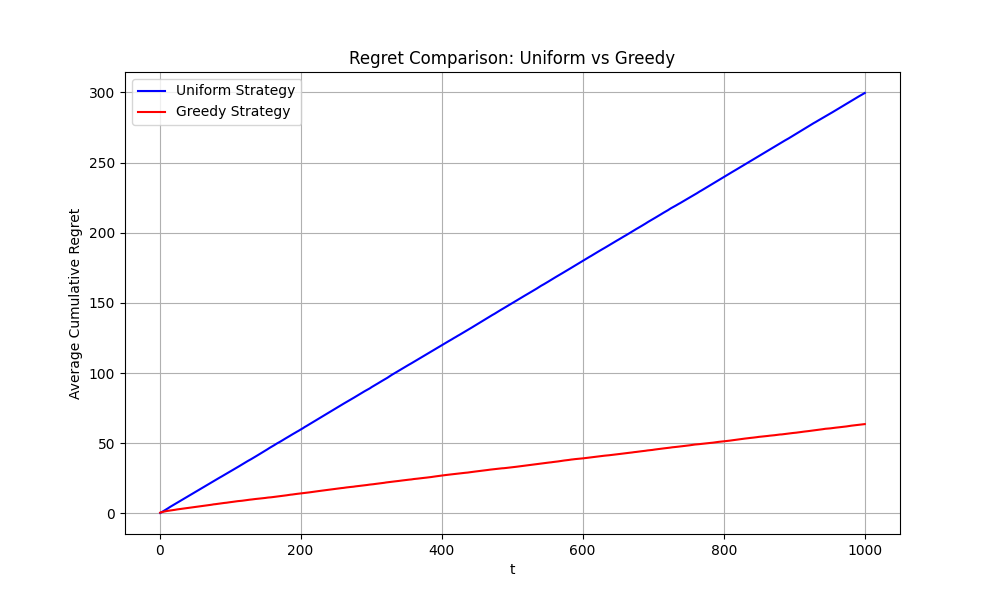
\includegraphics[width=0.8\textwidth]{regret_plot.png} 
    \caption{Regret Comparison: Uniform vs Greedy Strategy}
\end{figure}
Generally, the cumulative regret for both strategies appears to grow linearly.
However, the greedy strategy clearly performs better because it values exploitation and does not choose arms blindly (it improves its performance based on past data).
%

\section*{Theory Question 6} %
Given the uniform policy, the indicator variable $\mathbb{I}\{A_t = i\}$ follows: %
\[
\mathbb{I}\{A_t = i\} \sim \mathrm{Ber}\left(\frac{1}{k}\right)
\] %
Therefore: %
\[
N_i(T) = \sum_{t=1}^T \mathbb{I}\{A_t = i\} \sim \mathrm{Bin}\left(T, \frac{1}{k}\right)
\] %
\[
\mathrm{Regret}(T) = \sum_{i=1}^k \Delta_i \mathbb{E}[N_i(T)] = \sum_{i=1}^k \Delta_i \mathbb{E}\left[\mathrm{Bin}\left(T, \frac{1}{k}\right)\right] = \frac{T}{k} \sum_{i=1}^k \Delta_i
\] %
Using the given parameters, the regret is: %
\[
\mathrm{Regret}(1000) = \frac{1000}{2} (0 + 0.3) = 150
\] %
Obviously, if we strictly followed a policy that only chose the optimal arm, the regret would be zero.
The uniform strategy is sub-optimal because observing the result of an arm pull provides information about that arm's parameter.
As information accumulates, a rational agent should lean towards finding and exploiting the optimal arm.
The uniform policy acts completely blind and ignores this incoming data.
%

\section*{Theory Question 7} %
Suppose after the first two rounds, the empirical mean of the optimal arm ($\mu_1 = 0.9$) is lower than the sub-optimal arm ($\mu_2 = 0.6$) due to bad luck.
If $T=1000$, pure exploitation (Policy A) would lock onto the wrong arm early, creating a massive regret difference.
%
Thus, Policy A is not always better. While it yields zero regret if it luckily picks the correct arm, Policy B guarantees a linear regret of 150. However, if Policy A makes a mistake, its regret is significantly worse.
If we allocate the first 100 rounds for pure exploration, the Law of Large Numbers ensures empirical means closely match true means.
Then, exploiting for the remaining 900 rounds minimizes the total regret securely (a 1-to-9 exploration-to-exploitation ratio).
%

\section*{Theory Question 8} %
According to Hoeffding's inequality for $c_n(\delta)$: %
\[
P(|Y_n - \mu| \geq c_n(\delta)) \leq 2 \exp\left( -2n \left(\sqrt{\frac{\ln(2/\delta)}{2n}}\right)^2 \right) = \delta
\] %
\[
\implies P(|Y_n - \mu| < c_n(\delta)) = 1 - P(|Y_n - \mu| \geq c_n(\delta)) \geq 1 - \delta
\] %
This inequality bounds the probability of $Y_n$.
(The probability that the true mean lies within the confidence interval $[Y_n - c_n(\delta) , Y_n + c_n(\delta)]$ is $1-\delta$).
%
In a pure exploitation strategy, we seek to maximize $\mu_{i,t}$.
However, exploration is crucial in early stages.
The Upper Confidence Bound expression $\mu_{i,t} + c_{i,t}$ perfectly satisfies both needs.
Because:
a) For small $t$, the confidence interval $c_{i,t}$ is large.
Choosing the arm maximizing $\mu_{i,t} + c_{i,t}$ favors arms that have been played less (the bonus $c_{i,t}$ grows with $\ln t$ but shrinks as $N_{i,t}$ grows, so it stays large for rarely played arms), fulfilling the exploration objective.
%
b) For large $t$, $c_{i,t}$ shrinks, seamlessly transitioning the focus back to exploitation while still maintaining a tiny amount of exploration to reduce uncertainty.
%
Hence, selecting the arm that maximizes $\mu_{i,t} + c_{i,t}$ creates an elegant and effective balance between exploration and exploitation.
%

\section*{Simulation Question 2} %
\begin{figure}[htbp]
    \centering
    % Ensure hoeffding_plot.png is in the same directory
    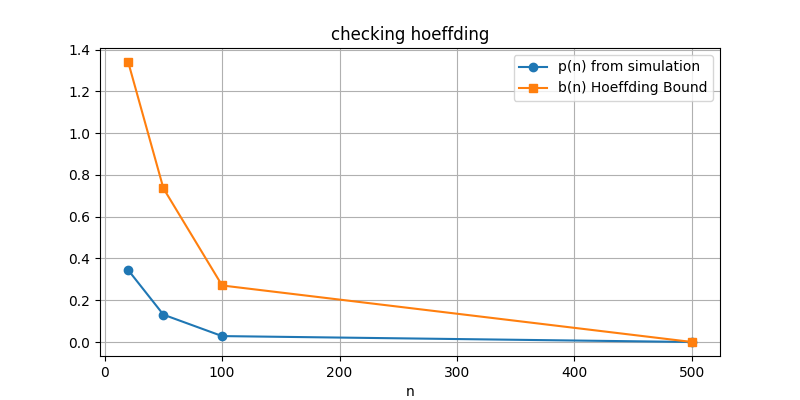
\includegraphics[width=0.8\textwidth]{hoeffding_plot.png} 
    \caption{Checking Hoeffding Bound}
\end{figure}
As observed in the plot, $p(n) \leq b(n)$ holds for every $n$, as Hoeffding's inequality guarantees (for $n=20$ the bound exceeds 1 and is therefore trivial).
However, as $n$ increases, the decay rate of the empirical probability and the theoretical bound align closely, causing them to converge and occasionally equalize.
%

\section*{Theory Question 9} %
\[
P(\mu_i) = \mathrm{Beta}(\alpha_i, \beta_i) \propto \mu_i^{\alpha_i - 1} (1 - \mu_i)^{\beta_i - 1}
\] %
\[
P(\mu_i | H_t) \propto P(H_t | \mu_i) P(\mu_i) \propto \mu_i^{\alpha_i - 1} (1 - \mu_i)^{\beta_i - 1} \mu_i^S (1 - \mu_i)^f \propto \mu_i^{\alpha_i + S - 1} (1 - \mu_i)^{\beta_i + f - 1}
\] %
\[
\implies P(\mu_i | H_t) = \mathrm{Beta}(\alpha_i + S, \beta_i + f)
\] %
As shown, the structural form of the posterior distribution is identical to the prior.
This proves that the Beta distribution is the conjugate prior for the Bernoulli likelihood.
The primary advantage of a conjugate prior is algebraic convenience, completely bypassing the need for complex integral calculations.
%

\section*{Simulation Question 3}
\begin{figure}[htbp]
    \centering
    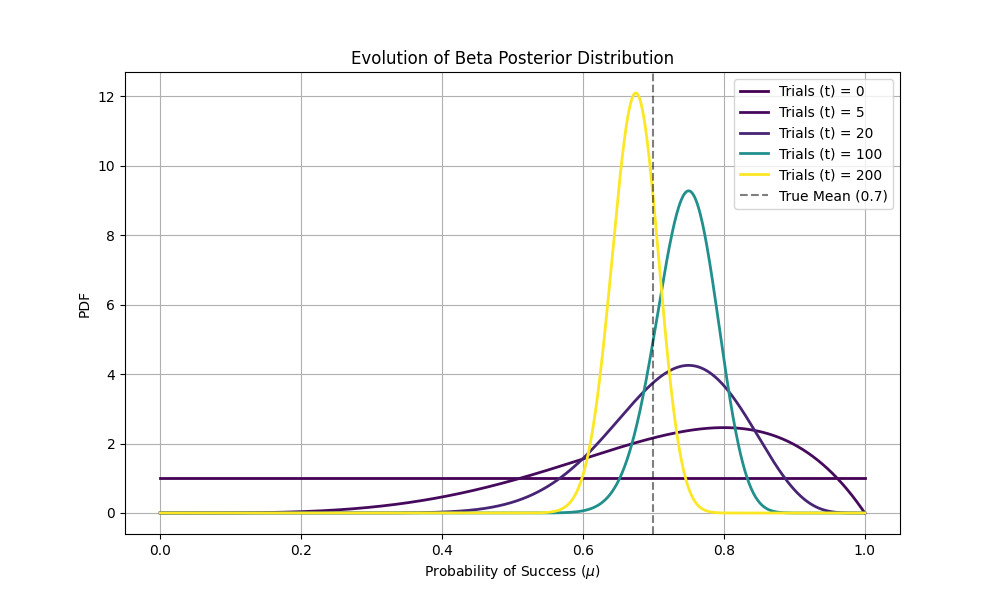
\includegraphics[width=0.8\textwidth]{Figure_3.png} 
    \caption{Evolution of Beta Posterior Distribution}
\end{figure}
As can be seen, with the increase in time steps, our PDF becomes sharper and more concentrated around the mean (its variance decreases).

\section*{Theory Question 10} %
The derivation follows the exact same logic as above.
We just need to account for the distribution coefficient to find the relation.
Ultimately, the core structure remains $\mathrm{Beta}(\alpha + S, \beta + f)$.
%

\section*{Simulation Question 4}
\begin{figure}[htbp]
    \centering
    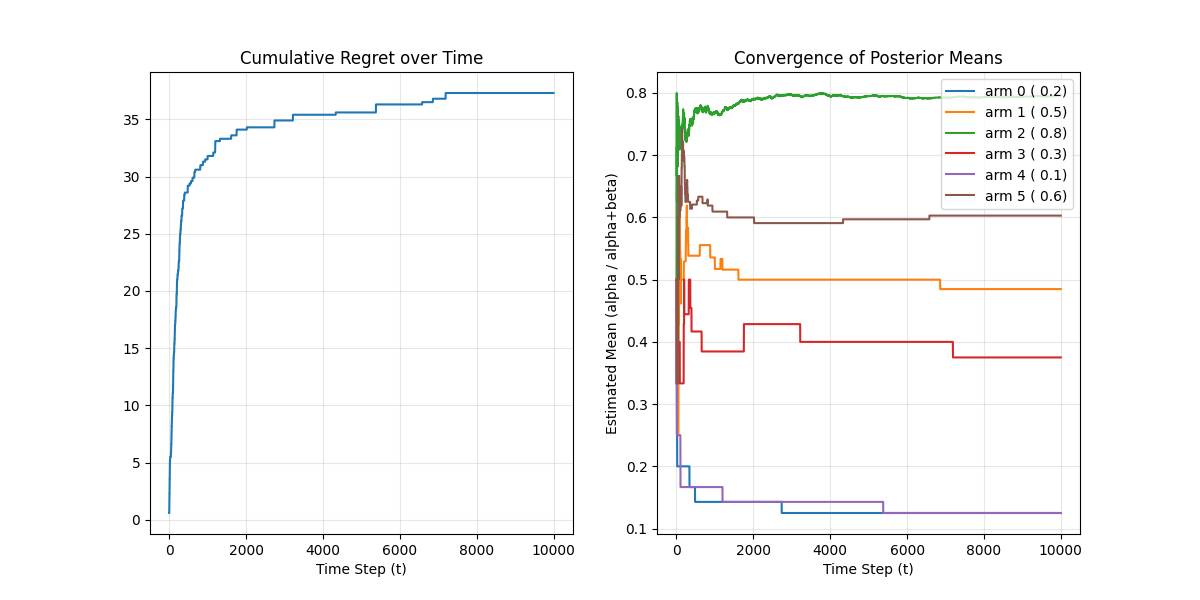
\includegraphics[width=1\textwidth]{Figure_4.png} 
    \caption{Cumulative Regret and Convergence of Posterior Means}
\end{figure}
As observed in the left graph, the regret of the TS algorithm grows logarithmically. In the right graph, we can observe the empirical means of the arms approaching their true means. (It is clear that they do not converge exactly to those values, especially the weaker arms, which lose their value after some exploration and are explored less over time).

\section*{Theory Question 11} %
In the Beta-Bernoulli Bayesian model, after observing the data, our belief distribution regarding the reward parameter is updated to a Beta posterior distribution $\mathrm{Beta}(\alpha', \beta')$.
The Probability Density Function (PDF) of this distribution is defined as follows: %
\[ 
f(\mu; \alpha', \beta') = \frac{1}{B(\alpha', \beta')} \mu^{\alpha'-1}(1-\mu)^{\beta'-1} 
\] %
where $B(\alpha', \beta')$ is the Beta function, calculated as: %
\[ 
B(\alpha', \beta') = \int_{0}^{1} t^{\alpha'-1}(1-t)^{\beta'-1} dt = \frac{\Gamma(\alpha')\Gamma(\beta')}{\Gamma(\alpha'+\beta')} 
\] %
To calculate the expected value (mean) of the random variable, we have: %
\[ 
\mathbb{E}[\mu] = \int_{0}^{1} \mu \cdot f(\mu; \alpha', \beta') d\mu 
\] %
Substituting the density function into the integral: %
\[ 
\mathbb{E}[\mu] = \int_{0}^{1} \mu \cdot \frac{\mu^{\alpha'-1}(1-\mu)^{\beta'-1}}{B(\alpha', \beta')} d\mu = \frac{1}{B(\alpha', \beta')} \int_{0}^{1} \mu^{\alpha'}(1-\mu)^{\beta'-1} d\mu 
\] %
The term inside the integral is the definition of the Beta function with parameters $\alpha'+1$ and $\beta'$: %
\[ 
\mathbb{E}[\mu] = \frac{B(\alpha'+1, \beta')}{B(\alpha', \beta')} 
\] %
Using the relationship between the Beta and Gamma functions, we expand the above expression: %
\[ 
\mathbb{E}[\mu] = \frac{\frac{\Gamma(\alpha'+1)\Gamma(\beta')}{\Gamma(\alpha'+1+\beta')}}{\frac{\Gamma(\alpha')\Gamma(\beta')}{\Gamma(\alpha'+\beta')}} = \frac{\Gamma(\alpha'+1)}{\Gamma(\alpha')} \cdot \frac{\Gamma(\alpha'+\beta')}{\Gamma(\alpha'+\beta'+1)} 
\] %
Using the recursive property of the Gamma function, i.e., $\Gamma(z+1) = z\Gamma(z)$, we will have: %
\[ 
\Gamma(\alpha'+1) = \alpha'\Gamma(\alpha') \quad \text{and} \quad \Gamma(\alpha'+\beta'+1) = (\alpha'+\beta')\Gamma(\alpha'+\beta') 
\] %
Substituting these values into the mean equation: %
\[ 
\mathbb{E}[\mu] = \frac{\alpha'\Gamma(\alpha')}{\Gamma(\alpha')} \cdot \frac{\Gamma(\alpha'+\beta')}{(\alpha'+\beta')\Gamma(\alpha'+\beta')} 
\] %
Finally, by simplifying the similar terms, the mean of the posterior distribution is obtained: %
\[ 
\mathbb{E}[\mu] = \frac{\alpha'}{\alpha'+\beta'} 
\] %

\section*{Theory Question 12} %
To calculate the probability of success in the next trial given past data, we use the Posterior Predictive Distribution.
This probability is obtained by averaging over the parameter: %
\[ 
P(X_{t+1} = 1 | \text{data}) = \int_{0}^{1} P(X_{t+1} = 1 | \mu) f(\mu | \text{data}) d\mu 
\] %
Given that $P(X_{t+1} = 1 | \mu) = \mu$ and our posterior distribution is $f(\mu | \text{data}) = \mathrm{Beta}(\alpha, \beta)$, we have: %
\[ 
P(X_{t+1} = 1 | \text{data}) = \int_{0}^{1} \mu \frac{\mu^{\alpha-1}(1-\mu)^{\beta-1}}{B(\alpha, \beta)} d\mu 
\] %
This integral represents the expected value of the $\mathrm{Beta}(\alpha, \beta)$ distribution.
Therefore: %
\[ 
P(X_{t+1} = 1 | \text{data}) = \frac{\alpha}{\alpha+\beta} 
\] %
\textbf{Analysis in the Context of Sequential Decision Making:} %
In sequential decision-making processes like Multi-Armed Bandits, this result shows that our best prediction for the future success rate of an arm is exactly the mean of our current belief distribution.
This value acts as a criterion for selecting arms in greedy algorithms.
As the number of observations increases (increasing the weight $\alpha+\beta$), the real data heavily outweighs the prior beliefs, and our prediction converges closer to the arm's true physical reality.
%

\section*{Theory Question 13} %
\textbf{Data:} %
First arm $\sim \mathrm{Beta}(2, 3)$ %
Second arm $\sim \mathrm{Beta}(10, 5)$ %

\textbf{Calculations:} %
Means: %
\[ 
\mathbb{E}[\mu_1] = \frac{2}{2+3} = 0.4 \quad , \quad \mathbb{E}[\mu_2] = \frac{10}{10+5} \approx 0.667 
\] %
Variances: %
\[ 
\mathrm{Var}(\mu_1) = \frac{2 \times 3}{(2+3)^2(2+3+1)} = \frac{6}{150} = 0.04 
\] %
\[ 
\mathrm{Var}(\mu_2) = \frac{10 \times 5}{(10+5)^2(10+5+1)} = \frac{50}{3600} \approx 0.0139 
\] %

\textbf{Thompson Sampling Behavior:} %
\begin{enumerate}
    \item \textbf{Exploitation:} The mean of the second arm is higher ($0.667 > 0.4$). Therefore, Thompson Sampling tends to select the second arm more often.
%
    \item \textbf{Exploration:} The variance of the first arm is greater ($0.04 > 0.0139$), meaning it has higher uncertainty.
Thus, TS will occasionally still select the first arm.
%
\end{enumerate}
\textbf{Balance:} This algorithm automatically balances exploiting the best current estimate (the second arm) and reducing the uncertainty of the lesser-known arm (the first arm).
%

\section*{Simulation Question 5}
\begin{figure}[H]
    \centering
    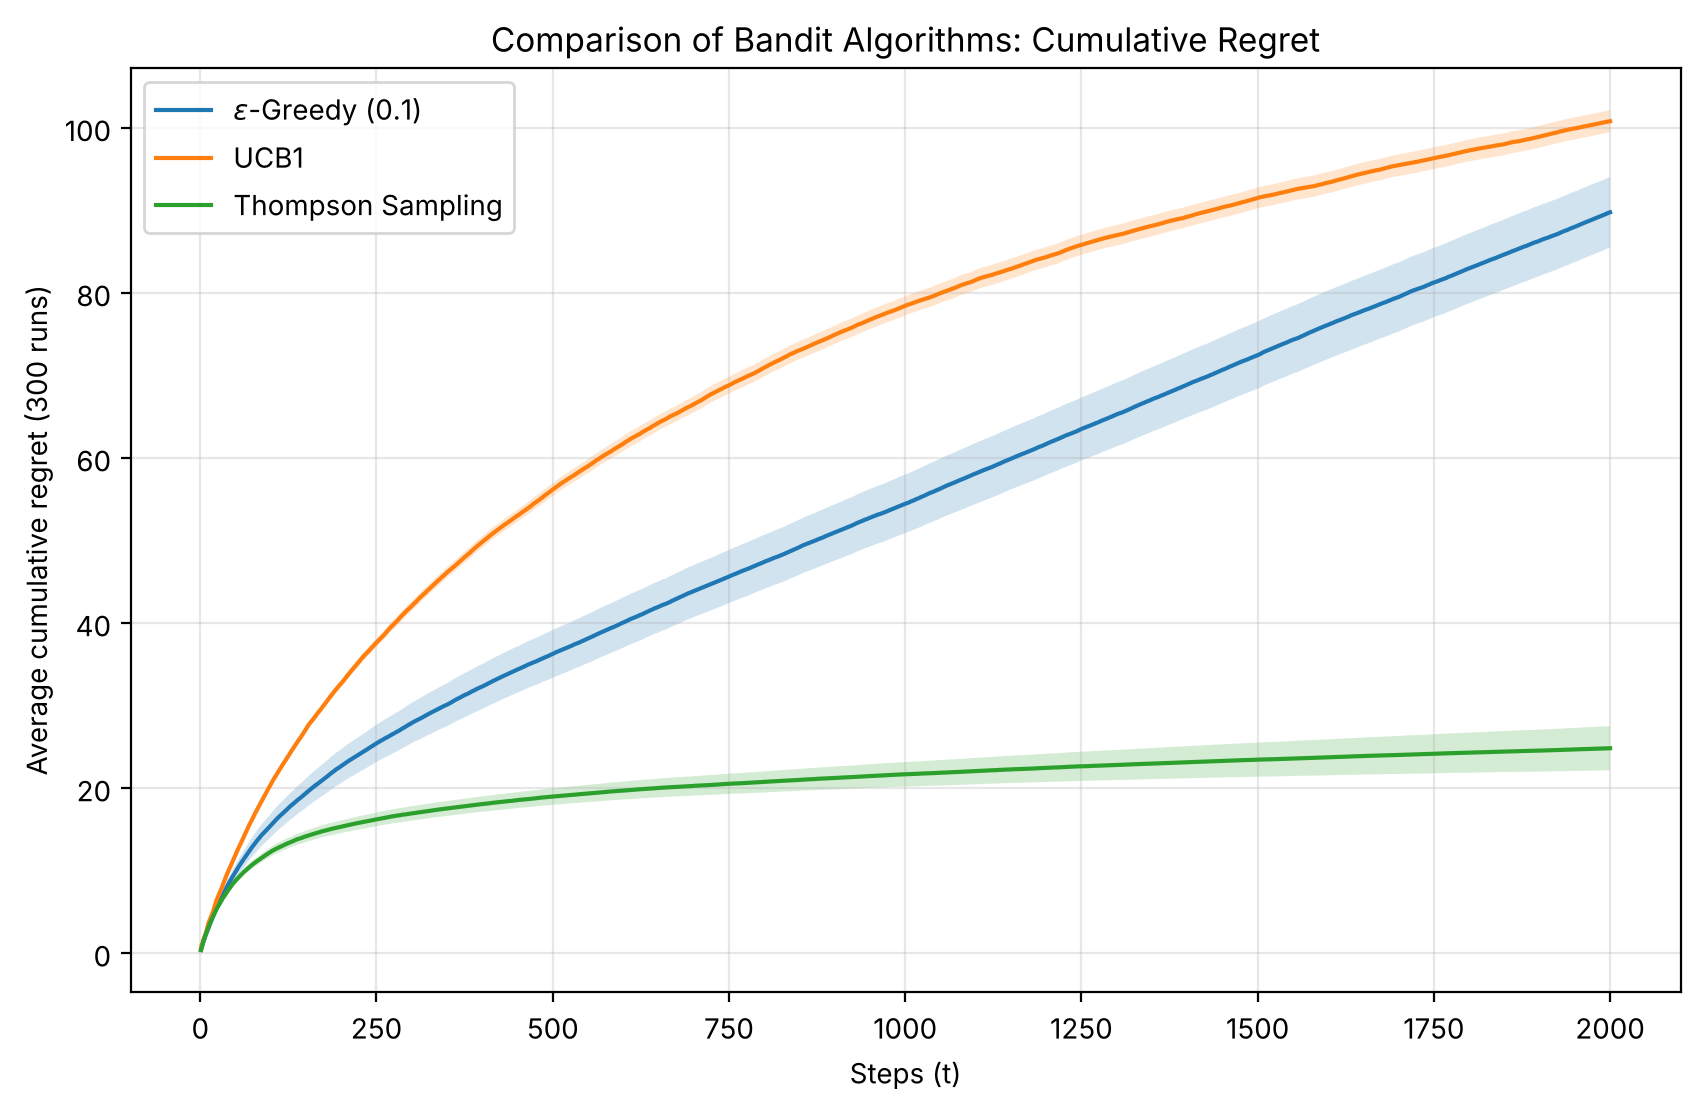
\includegraphics[width=1\textwidth]{Q5-bandit_algorithms_comparison.png} 
    \caption{Comparison of Cumulative Regret: $\epsilon$-Greedy, UCB, and Thompson Sampling}
\end{figure}

The curves are averages over 300 independent runs (shaded: 95\% confidence band). In every run the three algorithms face the same table of random rewards, so the comparison is not affected by luck in the rewards. Averaged regret at $T=2000$:
\begin{center}
\begin{tabular}{lc}
\hline
Algorithm & Regret at $T=2000$ \\
\hline
$\epsilon$-Greedy ($\epsilon=0.1$) & $89.7 \pm 4.3$ \\
UCB1 & $100.8 \pm 1.3$ \\
Thompson Sampling & $24.8 \pm 2.7$ \\
\hline
\end{tabular}
\end{center}
\textbf{Thompson Sampling} has by far the lowest regret. $\epsilon$-Greedy keeps exploring at a fixed rate, so after a short learning phase its regret grows linearly, with slope $\epsilon \cdot \frac{1}{k}\sum_i \Delta_i \approx 0.034$ per step. UCB1 grows only logarithmically, but its constant is large: the bonus $\sqrt{2\ln t / N_{i,t}}$ keeps the arms with means 0.5 and 0.3 in play for a long time. That is why UCB1 is still above $\epsilon$-Greedy at $T=2000$. A longer run (40 runs, $T=20000$) shows the crossing: at $T=5000$ the regrets are 132 (UCB1) and 191 ($\epsilon$-Greedy), and at $T=20000$ they are 178 and 703, against 34 for Thompson Sampling.

\section*{Theory Question 14} %
The Thompson Sampling (TS) algorithm achieves a dynamic balance between exploration and exploitation due to its Bayesian approach.
The reasons for achieving $\mathcal{O}(\log T)$ regret can be summarized as follows: %
\begin{enumerate}
    \item \textbf{Adaptivity:} In TS, the probability of choosing a sub-optimal arm decreases exponentially as the number of observations increases.
Unlike algorithms with a fixed exploration rate, TS only explores when there is uncertainty regarding the optimality of an arm.
%
    \item \textbf{Posterior Concentration:} As time $T$ increases, the variance of the posterior distribution for each arm approaches zero (for arm $i$ the posterior variance $\frac{\alpha\beta}{(\alpha+\beta)^2(\alpha+\beta+1)}$ falls roughly as $\mu_i(1-\mu_i)/N_i(t)$).
This concentration severely limits the probability of drawing large random samples from sub-optimal distributions, which would otherwise lead to choosing the wrong arm.
%
    \item \textbf{Matching the Lai-Robbins Bound:} It has been proven that the expected number of times a sub-optimal arm $i$ is chosen in the TS algorithm asymptotically satisfies: %
    \[ 
    \mathbb{E}[N_i(T)] \leq (1+\epsilon)\frac{\log T}{KL(\mu_i || \mu^*)} 
    \] %
    where $KL$ is the Kullback-Leibler divergence between the distribution of the sub-optimal arm and the optimal arm.
Since the total regret is derived from the relation $R(T) = \sum \Delta_i \mathbb{E}[N_i(T)]$, the final regret will be of the order $\mathcal{O}(\log T)$.
%
\end{enumerate}
Therefore, Thompson Sampling is considered an Asymptotically Optimal algorithm that achieves the most optimal possible learning rate.
%

\section*{Theory Question 15} %
The Probability Matching principle states that an agent should select an arm with a probability equal to its belief that the arm is optimal.
If $\theta_j$ is the unknown parameter of arm $j$ and $H$ is the history of observations, this probability is: %
\[ 
\pi_i = P(\theta_i = \max_j \theta_j | H) = \int_{\Theta} \mathbb{I}(\theta_i = \max_j \theta_j) P(\theta | H) d\theta 
\] %
Assuming the posterior independence of arms, we have $P(\theta | H) = \prod_{j=1}^K P(\theta_j | H)$.
Explicitly calculating this multiple integral is highly complex. %

\textbf{The Role of Thompson Sampling as a Monte Carlo Method:} %
Thompson Sampling solves this integral using the Monte Carlo method with just a single sample ($n=1$) at each time step: %
\begin{enumerate}
    \item For each arm, a sample $\hat{\theta}_j$ is drawn from the posterior distribution $P(\theta_j | H)$.
%
    \item The arm $A_t = \arg\max_j \hat{\theta}_j$ is selected.
%
\end{enumerate}
With this single draw, the probability that arm $i$ is chosen is exactly $\pi_i$, so Thompson Sampling implements probability matching exactly, not approximately.
In other words, the probability that the random sample of one arm is larger than the rest in a given time step is exactly equal to the value of the integral.
Thus, Thompson Sampling automatically implements probability matching without requiring heavy integration computations.
%

\section*{Simulation Question 6}
\begin{figure}[H]
    \centering
    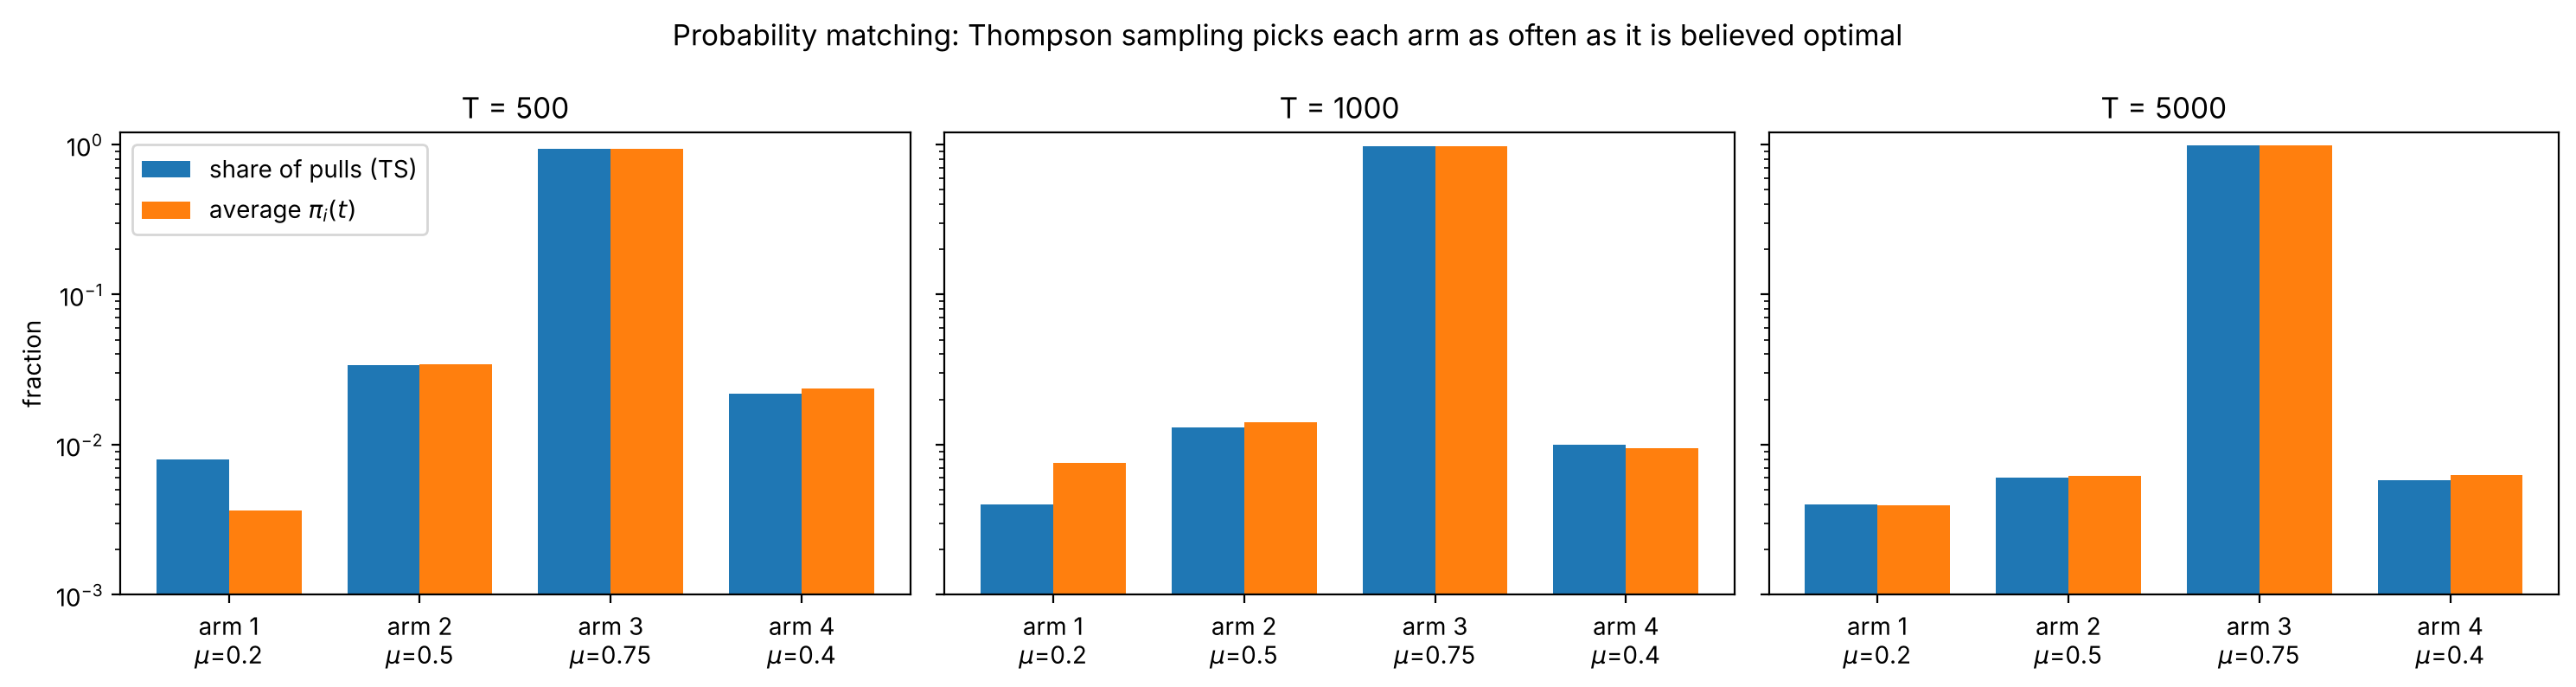
\includegraphics[width=1\textwidth]{Q6.png} 
    \caption{Share of pulls of each arm compared with the average posterior probability that the arm is optimal (log scale)}
\end{figure}

This simulation checks the connection between Thompson Sampling and \textbf{probability matching} from Theory Question 15. Probability matching states that, at every step, $P(A_t = i \mid H_t) = \pi_i(t)$, where $\pi_i(t) = P(\theta_i = \max_j \theta_j \mid H_t)$ is the posterior probability that arm $i$ is optimal. Taking the expectation of $\mathbb{I}\{A_t=i\}$ and summing over the run, the share of pulls of arm $i$ should equal the average of $\pi_i(t)$ over the same steps:
\[
\frac{1}{T}\sum_{t=1}^{T} \mathbb{I}\{A_t = i\} \;\approx\; \frac{1}{T}\sum_{t=1}^{T} \pi_i(t).
\]
At every step, before choosing an arm, the simulation estimates $\pi(t)$ by Monte Carlo, with 1000 joint draws from the Beta posteriors. Then it runs Thompson Sampling as usual. The two sides agree to within 0.004 for $T=500$ and $T=1000$, and to within 0.001 for $T=5000$. This holds for every arm, including the rarely played ones (see the log-scale bars).

Comparing the share of pulls with $\pi_i$ \emph{at the end} of the run, as an earlier version of this simulation did, is not a valid test. The final posterior describes only the last step, while the share of pulls averages over the whole run. Both vectors are also dominated by the best arm, so their correlation is close to 1 whatever the algorithm does.

\section*{Theory Question 16} %
The choice of the prior Beta distribution directly affects the balance between exploration and exploitation: %
\begin{enumerate}
    \item \textbf{Uniform Prior ($\mathrm{Beta}(1, 1)$):} This distribution is equivalent to $P(\mu) = 1$.
Due to its high variance ($\sigma^2 = 1/12$), it provides the maximum initial exploration.
The algorithm has no initial bias and is updated purely based on observed rewards.
%
    \item \textbf{Informative Prior ($\mathrm{Beta}(100, 100)$):} This prior represents overconfidence.
Its extremely small variance causes all samples to be concentrated around $0.5$.
This leads to under-exploration; the algorithm does not test new arms sufficiently because it assumes it already knows their means.
%
    \item \textbf{Jeffreys Prior ($\mathrm{Beta}(0.5, 0.5)$):} Theoretically, this distribution is invariant to reparameterization.
The concentration of density at the boundaries $0$ and $1$ causes the very first observation to have a severe impact on the posterior distribution.
This prior is suitable for quickly identifying extremely strong or extremely weak arms.
%
\end{enumerate}
\textbf{Conclusion:} In the absence of prior knowledge, $\mathrm{Beta}(1, 1)$ exhibits the most stable behavior, whereas $\mathrm{Beta}(100, 100)$ can cause the algorithm to get stuck in an incorrect estimate for a long time.
%

\section*{Simulation Question 7}
\begin{figure}[H]
    \centering
    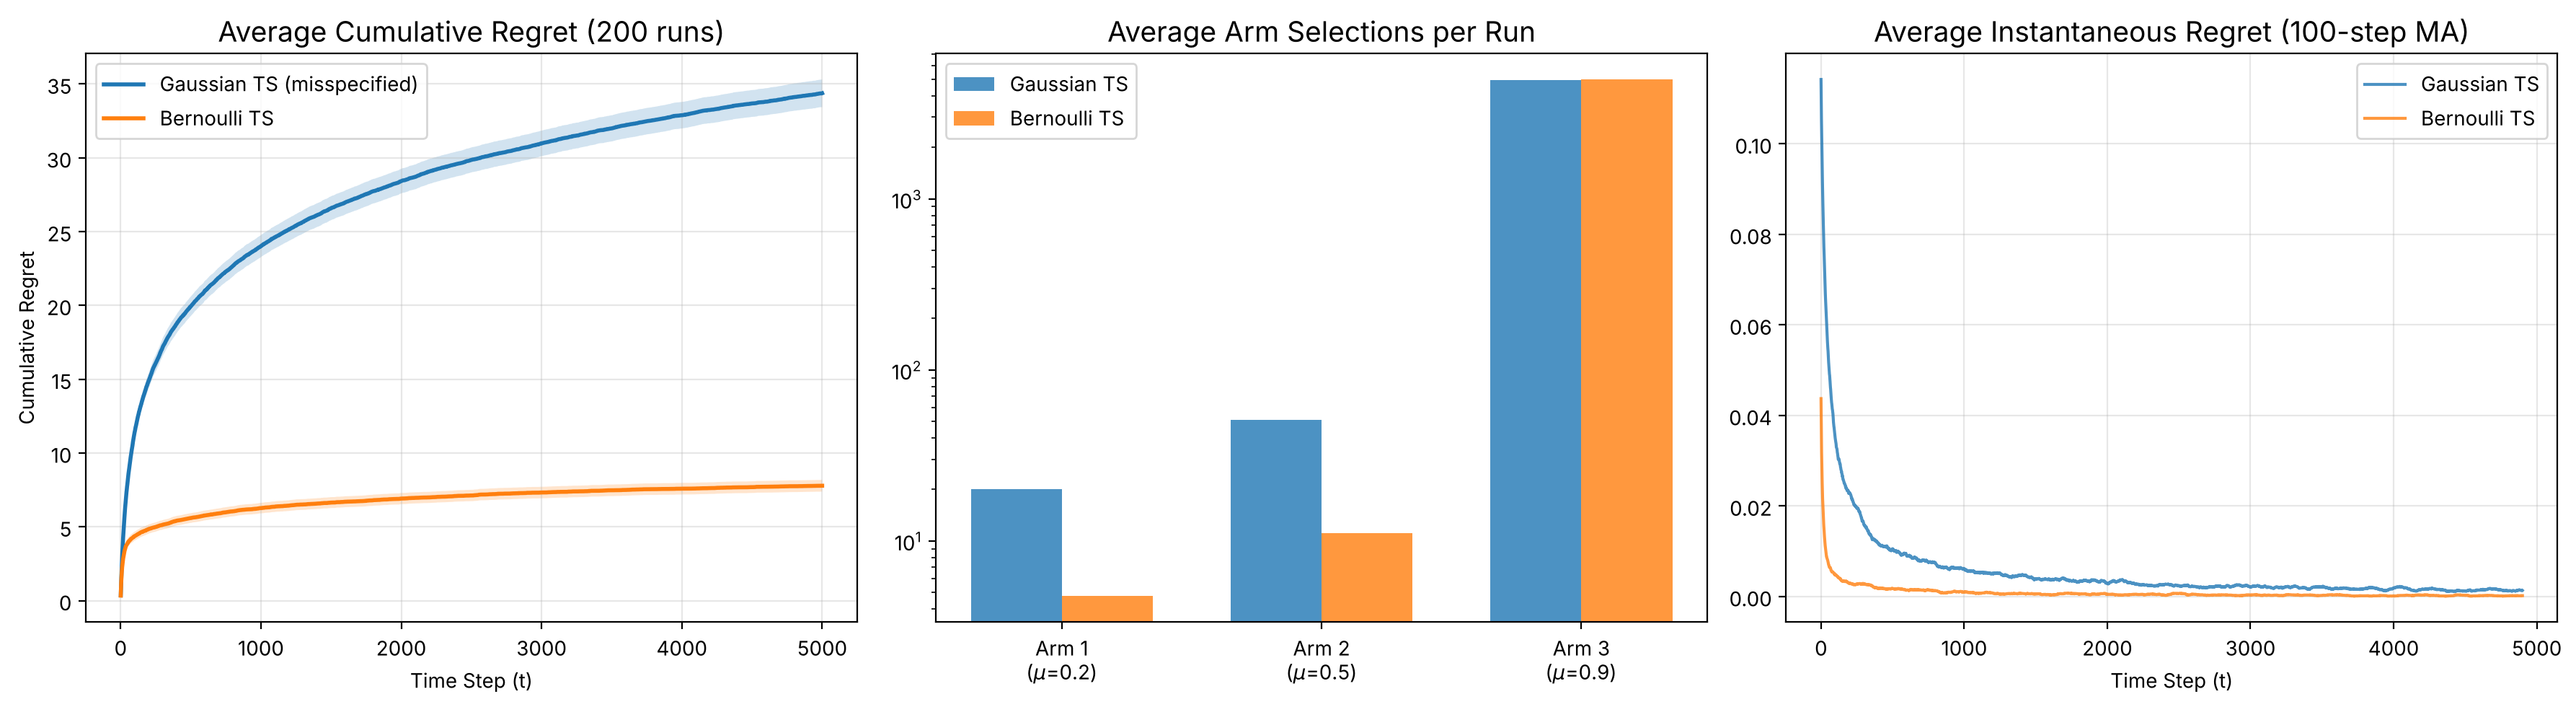
\includegraphics[width=1\textwidth]{Q7-gaussian_vs_bernoulli.png} 
    \caption{Comparison of Gaussian vs. Bernoulli Likelihoods in Thompson Sampling}
\end{figure}

This simulation compares two versions of Thompson Sampling on the \emph{same} Bernoulli bandit (means 0.2, 0.5 and 0.9). The rewards are binary, and in each of the 200 runs both algorithms see the same table of rewards.
\begin{itemize}
    \item \textbf{Bernoulli TS} uses the correct model: a Beta(1,1) prior and Beta--Bernoulli updates.
    \item \textbf{Gaussian TS} uses a misspecified model: a $\mathcal{N}(0,10)$ prior and a Normal likelihood with assumed variance $\sigma^2 = 1$, i.e.\ it treats the 0/1 rewards as noisy continuous values.
\end{itemize}
Results at $T=5000$ (mean $\pm$ 95\% CI): regret $34.4 \pm 0.9$ for Gaussian TS and $7.8 \pm 0.4$ for Bernoulli TS. The best arm receives 98.6\% and 99.7\% of the pulls.

Both algorithms find the best arm, but the Gaussian model explores more. A Bernoulli reward has variance $\mu(1-\mu) \le 0.25$, while the model assumes $\sigma^2 = 1$. Its posteriors therefore shrink as $1/N_i$ instead of as $\mu(1-\mu)/N_i$, so they stay too wide, and sub-optimal arms keep being sampled; arm 2 is pulled about five times as often. The price of the misspecification is about four times the regret.

An earlier version of this simulation drew the Gaussian algorithm's rewards from $\mathcal{N}(\mu_i, 1)$ instead of from the Bernoulli arms. The two algorithms were then solving different, unequally noisy problems, so that comparison did not measure the effect of the likelihood.

\end{document}